 %
\newcommand*{\MyIndentSit}{\hspace*{1 cm}}%

\chapter{Situering en doelstelling}
\label{Situering}
Het onderwerp van deze masterproef is: \newline
\MyIndentSit Geoptimaliseerde surveillance van een broadcaster voor real-time distribute van GNSS data stromen


Dit wordt onwikkeld samen met de Koninklijke Sterrenwacht van Belgi\"e. Voor het verder verloop van de masterproef, wordt hiernaar verwezen als de Royal Observatory of Belgium (ROB). Figuur \ref{imgROB} toont het logo van het ROB. De verdere uitleg over de situering van de masterproef staat in sectie \ref{SSit}.

\begin{figure}[hpb]
	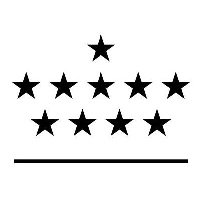
\includegraphics[scale=1]{ROB.jpg}
	\caption{Logo van de Koninklijke Sterrenwacht van Belgi\"e \cite{SImgROB}}
	\label{imgROB}
\end{figure} 

Het doel om het gebruik van data afkomstig van satellieten te bestuderen. Het doel wordt verder in detail besproken in sectie \ref{SDoe}.

\section{Situering}
\label{SSit}
Er zijn verschillende constellaties die deel uitmaken van het GNSS. In sectie \ref{LGNS} worden deze verder in detail besproken. Deze constellaties zijn opbebouwd uit satellieten. De data van deze satellieten wordt verzameld door het EUREF Permanent Network (EPN), hierover is meer informatie te vinden in sectie \ref{LEPN}. Het ROB doet dienst als het centrale bureau van het EPN. Hierdoor zijn zij verantwoordelijk voor het beheer van de data. In deze masterproef wordt verder ingegaan op het beheer van deze data en de logfiles. Deze worden verzameld door de broadcaster die gebruikt wordt om de data verder te verspreiden naar bevoegde instanties. Voorafgaand was er nog geen onderzoek gebeurd naar de logfiles van de broadcaster. Na de masterproef zou het voor de medewerkers van het ROB duidelijk moeten zijn wat er in de logfile staat. Dit moet grafisch weergegeven worden. Eveneens zou voor de verantwoordelijke het dagelijks beheer hierdoor eenvoudiger moeten worden. 

\section{Doel}
\label{SDoe}
Deze masterproef heeft volgende onderzoeksvraag: \newline
\MyIndentSit Welke gegevens worden door het logging systeem van de GNSS broadcaster verzameld? \newline
\MyIndentSit Is het mogelijk om met deze gegevens het beheer van de GNSS broadcaster te vergemakkelijken?\newline
\MyIndentSit Welke aanpassingen moeten in de software gebeurden zodat de doelstellingen verwezenlijkt kunnen worden? 
In de literatuurstudie (in hoofdstuk \ref{Literatuurstudie}) wordt in de eerste plaats gekeken naar de nodige kennis over satellieten, GNSS en de communicatie, om het practisch gedeelte van de masterproef te kunnen begrijpen.
\newline
Deze masterproef heeft als uiteindelijk doel een nieuw geoptimaliseerd logging systeem voor de GNSS broadcaster te ontwerpen. Deze broeadcaster moet uiteindelijk in staat zijn om:
\begin{itemize}
	\item Detecteren en reageren op potenti\"ele beveiligings problemen. (Zoals bijvoorbeeld herhaaldelijk proberen aanmelden met een verkeerd paswoord, veel simultane verbindingen ...)
	\item Feedback geven aan de leveranciers van datastromen over het gebruik van hun data
	\item Bestuderen van de status/gezondheid van clients, sofware gebruikt voor het maken van de verbinding, het gebruikt protocol, verbruik van de bandbreedte ...
\end{itemize}
Het zou kunnen dat om dit te verwezelijken de software van de logger aangepast moet worden zodat er meer data bewaart wordt. De verkregen informatie moet grafisch worden voorgesteld op een web-gebaseerde interface.  Deze interface moet voor de verantwoordelijke van de configuratie van de broadcaster het dagelijks beheer vergemakkelijken. 